\documentclass[9pt,twocolumn,twoside,]{pnas-new}

%% Some pieces required from the pandoc template
\providecommand{\tightlist}{%
  \setlength{\itemsep}{0pt}\setlength{\parskip}{0pt}}

% Use the lineno option to display guide line numbers if required.
% Note that the use of elements such as single-column equations
% may affect the guide line number alignment.


\usepackage[T1]{fontenc}
\usepackage[utf8]{inputenc}


\templatetype{pnasresearcharticle}  % Choose template

\title{Culture in oranzees}

\author[a,1]{Alberto Acerbi}
\author[b]{William Snyder}
\author[b]{Claudio Tennie}

  \affil[a]{Centre for Culture and Evolution, Department of Life Sciences, Brunel
University London, Uxbridge, UB8 3PH, United Kingdom}
  \affil[b]{Faculty of Science, Department for early prehistory and quaternary
ecology, University of Tübingen, Schloß Hohentuebingen, Burgsteige 11,
72070, Tübingen, Germany}


% Please give the surname of the lead author for the running footer
\leadauthor{Acerbi}

% Please add here a significance statement to explain the relevance of your work
\significancestatement{Authors must submit a 120-word maximum statement about the significance
of their research paper written at a level understandable to an
undergraduate educated scientist outside their field of speciality. The
primary goal of the Significance Statement is to explain the relevance
of the work in broad context to a broad readership. The Significance
Statement appears in the paper itself and is required for all research
papers.}


\authorcontributions{Please provide details of author contributions here.}

\authordeclaration{Please declare any conflict of interest here.}


\correspondingauthor{\textsuperscript{} }

% Keywords are not mandatory, but authors are strongly encouraged to provide them. If provided, please include two to five keywords, separated by the pipe symbol, e.g:
 \keywords{  cultural transmission |  cultural evolution |  cumulative culture |  non-human great ape culture |  individual-based models |  animal culture  } 

\begin{abstract}
Please provide an abstract of no more than 250 words in a single
paragraph. Abstracts should explain to the general reader the major
contributions of the article. References in the abstract must be cited
in full within the abstract itself and cited in the text.
\end{abstract}

\dates{This manuscript was compiled on \today}
\doi{\url{www.pnas.org/cgi/doi/10.1073/pnas.XXXXXXXXXX}}

\begin{document}

% Optional adjustment to line up main text (after abstract) of first page with line numbers, when using both lineno and twocolumn options.
% You should only change this length when you've finalised the article contents.
\verticaladjustment{-2pt}

\maketitle
\thispagestyle{firststyle}
\ifthenelse{\boolean{shortarticle}}{\ifthenelse{\boolean{singlecolumn}}{\abscontentformatted}{\abscontent}}{}

% If your first paragraph (i.e. with the \dropcap) contains a list environment (quote, quotation, theorem, definition, enumerate, itemize...), the line after the list may have some extra indentation. If this is the case, add \parshape=0 to the end of the list environment.

\acknow{This project has received funding from the European Research Council
(ERC) under the European Union's Horizon 2020 research and innovation
programme (grant agreement n° 714658; STONECULT project). We would like
to than Mima Batalovic, ETC.}

Cumulative culture, the transmission and improvement of knowledge,
technologies, and beliefs from individual to individual, and from
generation to generation, is key to explain the extraordinary ecological
success of our species (1, 2). Which cognitive abilities underpin
human's cumulative cultural capacities, and how these abilities affect
the evolution of culture itself are among the most pressing question of
evolutionary human science.

Many other species, besides humans, are able to at least use social cues
to modify their behaviour. Various primates have shown to posses complex
traditions that are socially influenced (3--5). Differently from other
primate species, however, humans have cumulative culture. While there
are various definitions of cumulative culture (6), some of its
characteristics are broadly accepted. Cumulative culture requires the
accumulation of cultural traits (more cultural traits are present at
time \emph{t} than at time \emph{t-1}), their improvement (more
effective cultural traits at time \emph{t} than at time \emph{t-1}), and
ratcheting (the innovation of cultural traits at time \emph{t} depends
on the presence of other traits at time \emph{t-1}) (7).

Not all human culture needs to be supported by faithful copying (8), but
our \emph{cumulative} culture depends on an ability to transmit and
preserve accurately \emph{new} information. Experiments have indeed
shown that humans are capable of copying, and that they routinely copy
cross-culturally. More controversial is the claim that other species
copy. Claims regarding the existence of non-human great ape cultures
based on copying raise a puzzling question: if other ape species can and
do copy, why do they not develop cumulative cultures? There are only two
possible answer to this question. Either they do not copy, or copying
does not automatically lead to cumulative culture.

Ape primatologists have claimed the existence of copying-based cultures
from outcomes of observations of wild populations. For example, (3)
examined the population-level distribution of behavioral traits in
populations of chimpanzees across seven sites, and argued that this
distribution proved the existence of copying-based cultures in these
populations. We developed an individual-based model to assess whether
these patterns actually warrant to pinpoint copying as the underlying
learning mechanism. We reproduced several details of the original study,
including realistic demographic and spatial features, and effects of
ecological availability and genetic predisposition, to investigate
whether an equivalent distribution of behavioral traits could emerge in
absence of any copying. While our simulated species, \emph{oranzees},
can be influenced by social cues (widespread in the animal kingdom, and
certainly present in all apes), we explicitly did not model any copying.

Our results show that, under realistic values of the main parameters, we
can reproduce the distribution of behavioral traits found in (3),
without any copying required. In other words, as oranzees can and do
show cultural patterns resembling wild ape patterns, this is proof that
such patterns cannot be counted as evidence that copying must have taken
place.

\section*{Materials and methods}\label{materials-and-methods}
\addcontentsline{toc}{section}{Materials and methods}

We built an individual-based model that reproduces a world inhabited by
six populations of ``oranzees'', a hypothetical ape species. The model
is space-explicit: the oranzees populations are located at relative
positions analogous to the six chimpanzees sites in (3). This is
important to determine the potential genetic predispositions and
ecological availabilities associated to their possible behaviours (see
below). Population sizes are also taken from the sites in (3). Following
(9), we use data from (10), and we define population sizes as
\(N=\{20;42;49;76;50;95\}\).

Oranzees are subject to an age-dependent birth/death process, broadly
inspired by descriptions in (11). A time step \(t\) of the simulation
represents a month in oranzees' life. From when they are 25 years old
(\(t=300\)), there is a 1\% probability an oranzee will die each month,
or they die when they are 60 years old (\(t=720\)). The number of
individuals in the population is fixed, so each time an oranzee dies it
is replaced by a newborn.

A newborn oranzee does not yet show any behaviour. Behaviours can be
innovated at each time step. The process of innovation is influenced by:
(i) the oranzees `state', which depends on the behaviours an individual
already possesses, (ii) the frequency of the behaviours already present
in the population (``socially-mediated reinnovation'' in (12)), and
(iii) the genetic propensity and ecological availability locally
associated to the behaviour. At the beginning of the simulations, the
populations are randomly initialised with individuals between 0 and 25
years old.

\subsection*{State}\label{format}
\addcontentsline{toc}{subsection}{State}

In the oranzees world, 64 behaviours are possible. Behaviours are
divided into two categories, namely 32 social and 32 food-related
behaviours. These figures where chosen to resemble the behavioural
categories considered in (3).

In the case of social behaviours, we assume four sub-categories (e.g.
`play', `groom', etc.), each with eight possible different behaviours,
that serve the same goal. Oranzees' state is based on how many of the
four goals are fulfilled. A goal is considered fulfilled if an oranzee
has at least one behaviour out of the eight in the sub-category. An
oranzee has a state value of \(0.25\) if, for example, it has at least
one behaviour among the first eight behaviour, and none of the others,
and a state value of \(1\) if there is at least one behaviour in each
sub-category. \(p_\text{social}\), the probability to innovate a social
behaviour, is drawn from a normal distribution with mean equal to
\(1-state_\text{social}\).

Food-related behaviours are analogously divided into sub-categories,
with the differences, with respect to social behaviours, that there is a
variable number of behaviours in each sub-category, and that
sub-categories are associated to two different `nutrients', \emph{Y} and
\emph{Z}. Here individuals need to balance their nutritional intake, so
that their optimal diet consist in a roughly equal number of food for
one and the other nutrient. The state, for food-related behaviours,
depends on the total amount of food ingested \emph{and} on the balance
between nutrients, and it is calculated as the sum of each sub-category
fulfilled (as above, for this to happen there needs to be at least one
behaviour present) minus the difference between the number of
sub-categories providing nutrient \emph{Y} and the number of
sub-categories providing nutrient \emph{Z}. We normalize the state
between \(0\) and \(1\), and, as above \(p_\text{food}\) is then
calculated as \(1-state_\text{food}\). (Further details in SI).

\subsection*{Socially-mediated reinnovation}\label{format}
\addcontentsline{toc}{subsection}{Socially-mediated reinnovation}

At each time step, all oranzees have a probability of innovation for
social and food-related behaviours calculated as described above. The
specific behaviour an oranzee will innovate depends both on the
frequency of the behaviours already present in the population, and on
the ecological availability and genetic propensity associated to the
behaviour. A further parameter of the model, \(S\), controls the
probability that each reinnovation is socially-mediated (12). When a
reinnovation is socially-mediated, the probability of innovating each
behaviour \(B_i\) is weighted by its proportional instances in the
population, among the behaviours of the same category, so that common
behaviours are more likely to be reinnovated.

When the reinnovation is not socially-mediated, the probability of
innovating each behaviour is random. Only one behaviour per category can
be innovated at each time step.

\subsection*{Genetic propensity and ecological
availability}\label{format}
\addcontentsline{toc}{subsection}{Genetic propensity and ecological
availability}

The behaviour selected in the previous step is then innovated or not
according to its genetic propensity and, in case of food-related
beahviours, ecological availability.

Genetic propensity is a probability \(p_g(0,1)\), assigned independently
for each of the 64 behaviours. A parameter of the model, \(\alpha_g\),
determines the probability that the genetic propensity of each behaviour
is equal for all the six populations or whether is different. If the
probability is equal, \(p_g\) is randomly drawn. If it is different, we
assign the propensity using a geographical gradient. We choose a random
point and calculate its distance to each population. Distances are then
transformed to \(p_g\) by rescaling them between 0 and 1, so that for
the farther site \(p_g=0\) i.e.~the associated behaviour will be
impossible to express (see SI). Notice that \(\alpha_g=0\) does not mean
that there are no genetic influences on the behaviour, but that there
are no \emph{differences} between the populations with regard to this
aspect.

Ecological availability is a probability \(p_e(0,1)\) that represents
the likelihood of finding a resource, or its nutritional value, in each
site. Ecological availability is assigned only to food-related
behaviours, and it is calculated in the same way of \(p_g\), using the
parameter \(\alpha_e\) to determine the probability of ecological
availability being different in the six populations.

\subsection*{Model's output}\label{format}
\addcontentsline{toc}{subsection}{Model's output}

We run simulations for \(t_\text{max}=6000\) (corresponding to 500 years
of oranzee-time). For each simulation, following (3), we classify each
behaviour, in each population, as:

\begin{itemize}
\item
  \emph{customary}: a behaviour observed in over 50\% of individuals in
  at least one age class (see SI for how age classes are defined in our
  model).
\item
  \emph{habitual}: a behaviour observed in at least two individuals
  across the population.
\item
  \emph{present}: a behaviour observed in at least one individual across
  the population.
\item
  \emph{absent}: a behaviour not observed even once in the population.
\item
  \emph{ecological explanations}: a behaviour that is absent because of
  complete lacking of local ecological availability (i.e., in our model,
  associated to \(p_e=0\)).
\end{itemize}

Notice the last category in (3) (\emph{unknown}, i.e. ``the behaviour
has not been recorded, but this may be due to inadequacy of relevant
observational opportunities'') does not apply in our case, because we
have full knowledge of the output of the simulations.

Finally, to test how well our model compares to the results in wild ape,
we calculate the same ``patterns'' described in (3):

\begin{itemize}
\item
  \emph{A}: behaviour absent at no site.
\item
  \emph{B}: behaviour not achieving habitual frequencies at any site.
\item
  \emph{C}: behaviour for which any absence can be explained by local
  ecological factors.
\item
  \emph{D}: behaviour customary or habitual at some sites yet absent at
  others, with no ecological explanation, i.e.~the behaviours defined as
  ``cultural''.
\end{itemize}

\section*{Results}\label{results}
\addcontentsline{toc}{section}{Results}

We are particularly interested in the realistic parameter conditions of
moderate to high environmental variability (\(\alpha_e=(0.5,1)\)) and
zero to moderate genetic differences (\(\alpha_g=(0,0.5)\)). We run 20
simulations for each combination (for a total of 600 runs). For all,
reinnovation is socially-mediated (\(S=1\)). The results show that
various combinations of parameters produces a number of cultural
behaviours (pattern \emph{D}) consistent with the 38 found in (3), in
absence of any explicit copying mechanism implemented (see Figure
\ref{Figure1}).

\begin{figure*}[h!]
\begin{center}
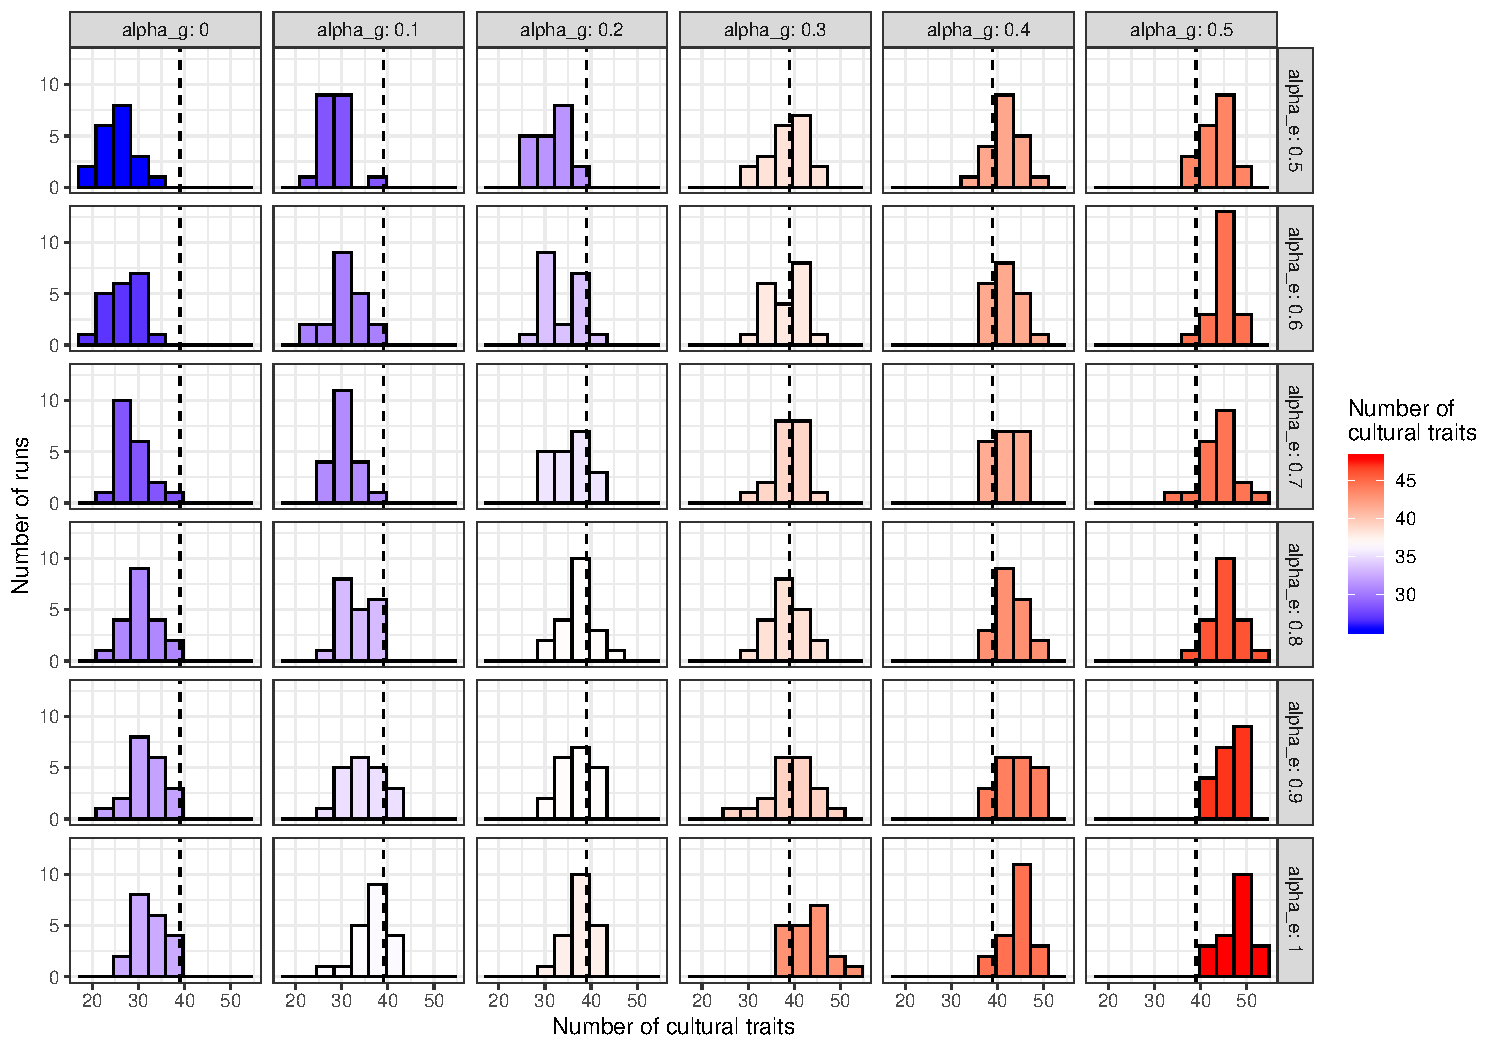
\includegraphics[width=17.8cm]{figures/figure_1.pdf}
\caption{Number of cultural traits in oranzees, when varying ecological and genetic diversity. Red colour indicates simulation runs that produced more than 38 cultural behaviours; blue colour indicates simulation runs that produces less than 38 cultural behaviours. For all simulations, $S=1$, $\alpha_e$ and $alpha_g=0$ as indicated in the plot. $N=20$ runs for each parameters combination.}
\label{Figure1}
\end{center}
\end{figure*}

We also analyse the effect of the parameter \(S\) (proportion of
socially-mediated reinnovations), in three conditions (see Figure
\ref{Figure2}): (a) no genetic differences and intermediate ecological
differences (compare to the high-left angle of Figure \ref{Figure1},
where with \(S=1\) simulations produce less than 38 cultural
behaviours), (b) good match with (3), and (c) intermediate genetic
differences and high ecological differences (compare to the low-right
angle of Figure \ref{Figure1}, where with \(S=1\) simulations produce
more than 38 cultural behaviours). As expected, decreasing \emph{S},
decreases the number of cultural behaviours. Conditions where, with
\(S=1\), there were more than 38 cultural behaviours could still produce
results analogous to (3), when not all reinnovations are socially
mediated.

\begin{figure*}[h!]
\begin{center}
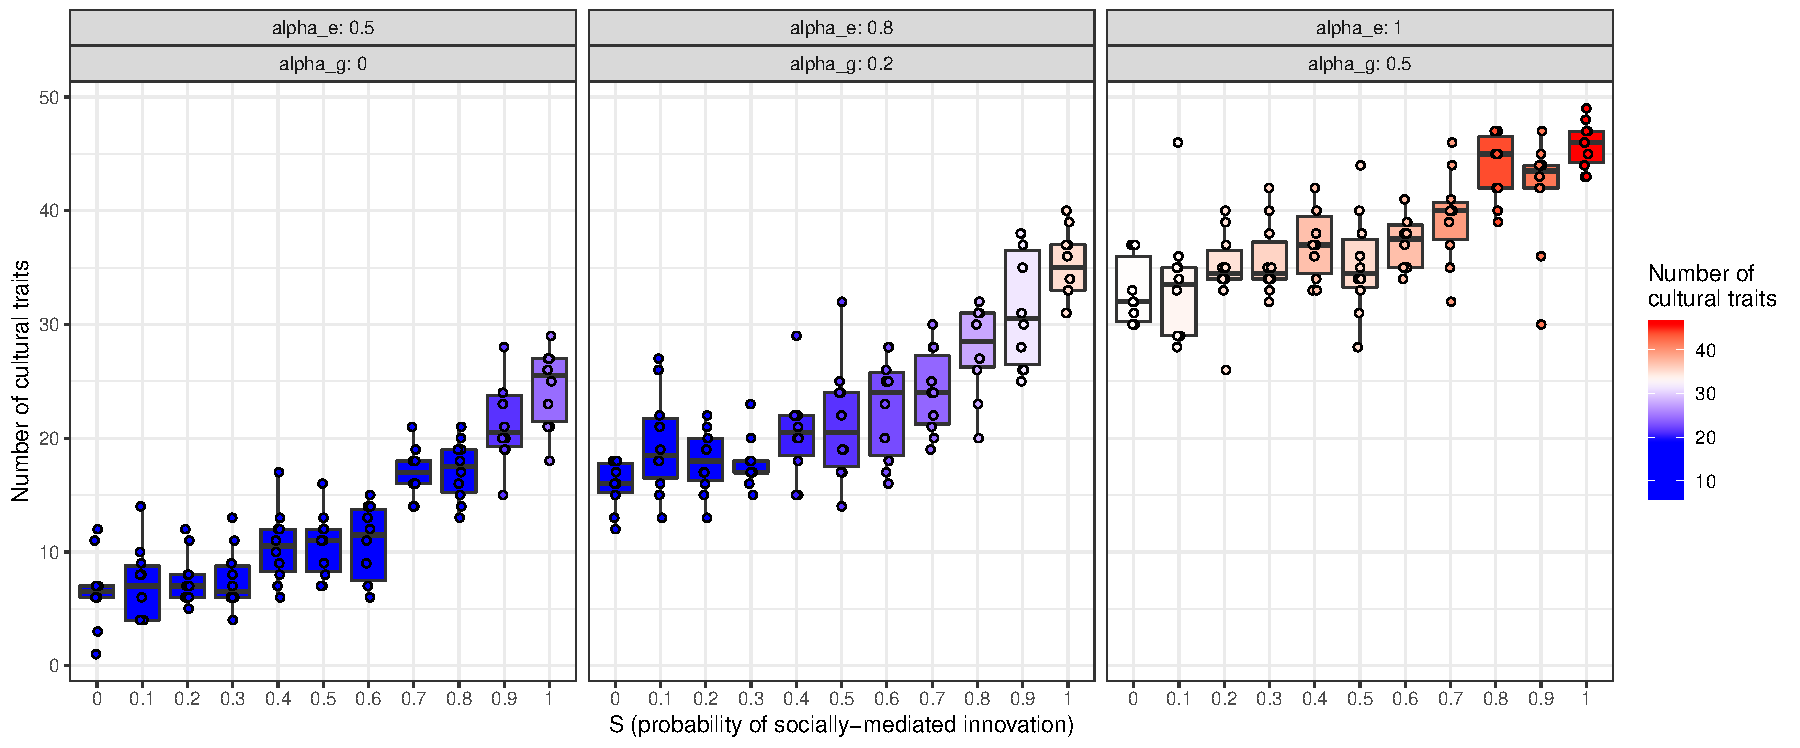
\includegraphics[width=17.8cm]{figures/figure_2.pdf}
\caption{Cultural traits in oranzees, varying the probability of socially-mediated innovations. Red colour indicates simulation runs that produced more than 38 cultural behaviours; blue colour indicates simulation runs that produces less than 38 cultural behaviours. $S$, $\alpha_e$ and $alpha_g=0$ as indicated in the plot. $N=10$ runs for each parameters combination.}
\label{Figure2}
\end{center}
\end{figure*}

Our results show that our model not only reproduces very well the number
of cultural behaviours (pattern \emph{D}), but also the number of
behaviours classified in the other three patterns (\emph{A}, \emph{B},
\emph{C}) in (3). Figure \ref{Figure3} show the four patterns produced
in one of the conditions for which we have a good match for cultural
behaviours (\(\alpha_e=0.8;\alpha_g=0.2, S=1\)).

\begin{figure*}[h!]
\begin{center}
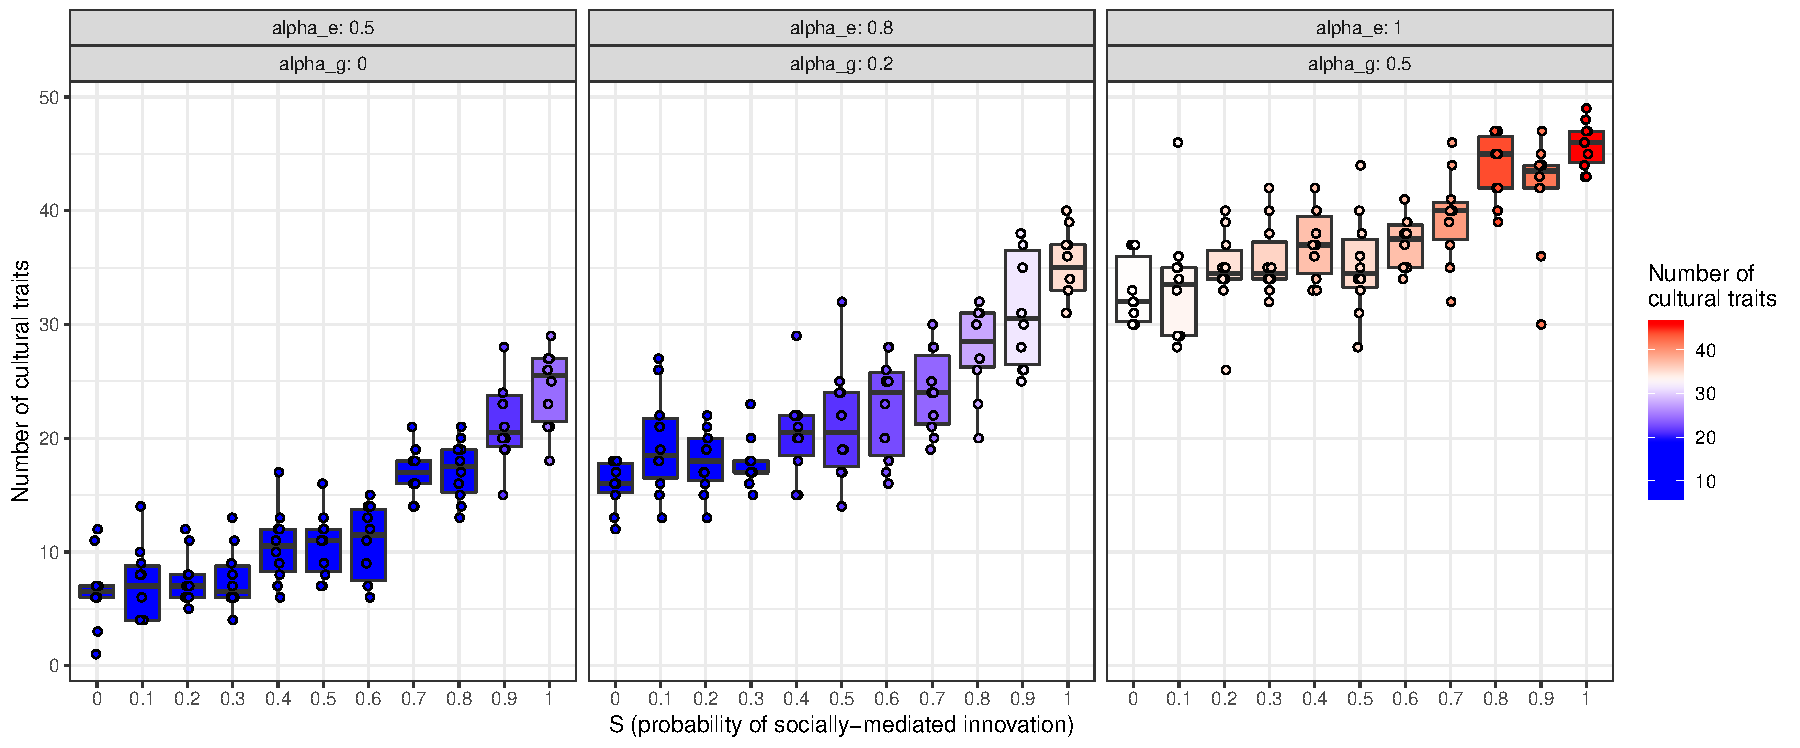
\includegraphics[width=11.4cm]{figures/figure_3.pdf}
\caption{Number of behaviours for each of the four patterns (*A*, *B*, *C*, *D*) for the parameters $\alpha_e=0.8;\alpha_g=0.2,S=1$. The red values are the values described for real chimpanzees populations. $N=20$ runs.}
\label{Figure3}
\end{center}
\end{figure*}

Finally, we run 100 simulations for the same condition where we have a
good match for cultural behaviours with (3)
(\(\alpha_e=0.8;\alpha_g=0.2, S=1\)). In each simulation, we recorded,
for each population, the number of behaviours (habitual + customary +
present) that are also classified as cultural (see Figure
\ref{Figure4}). We find a small, but significant, correlation between
population size and number of cultural traits
(\(p<0.00001,\rho=0.2,N=600\)). In other words, our model reproduces the
effect of cultural accumulation relative to population size possibly
found in real populations (compare (9, 13, 14)).

\begin{figure*}[h!]
\begin{center}
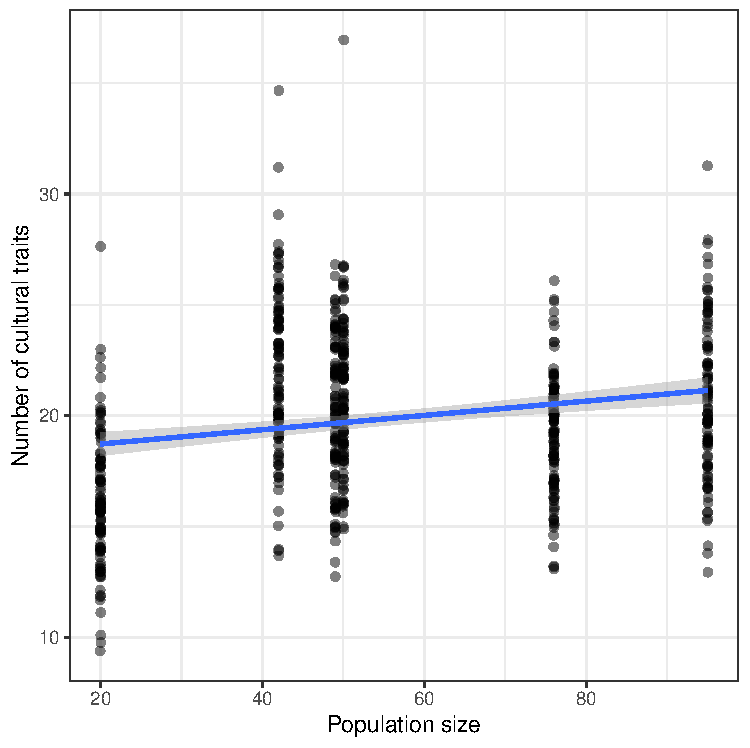
\includegraphics[width=11.4cm]{figures/figure_4.pdf}
\caption{Number of cultural behaviours for each population for the parameters $\alpha_e=0.8;\alpha_g=0.2,S=1$. The blue line is a linear fit of the data. $N=100$ runs.}
\label{Figure4}
\end{center}
\end{figure*}

\section*{Discussion}\label{discussion}
\addcontentsline{toc}{section}{Discussion}

We developed an individual-based model to examine under which conditions
a distribution of behavioral traits analogous to the distribution
reported in (3) in chimpanzees could emerge, crucially, without allowing
for the existence of any copying mechanism. We implemented several
details of the original study, including realistic demographic and
spatial features, as well as effects of genetic propensity and
ecological availability on the behaviours. Given the widespread
availability of non-copying variants of social learning, we also We also
included socially-mediated reinnovation, where social learning merely
catalyses individual reinnovation (12).

Our main result is that we can reproduce the wild ape pattern under
realistic values of the parameters of genetic propensity and ecological
availability, namely null to medium importance of genetic variation, and
medium to high importance of ecological variation. While we cannot
precisely pinpoint the exact values that these parameters should have to
reproduce real population of chimpanzees (or other apes), we are
confident that the range of values explored, and the relative ease by
which patterns of cultural behaviours similar to (3) can be produced in
the model, strongly suggest that copying is not required for those
patterns to emerge. Therefore, ape-like cultural patterns do not and
cannot pinpoint copying abilities or necessities. In addition, and as
further support to our results, our model not only reproduces the
cultural behaviours pattern, but also the proportions among the other
patterns, i.e.~absent behaviours, behaviours not achieving habitual
frequencies at any site, and behaviours absent because of ecological
factors.

In our model, we focused on the mechanism of socially mediated
reinnovation, that is, we assumed that members of our hypothetical
species, oranzees, had a probability to reinnovate a specific behaviour
stochastically linked to how many other oranzees in the population were
already showing this behaviour. While this is a realistic assumption
(15) and it reproduces in our model the chimpanzees cultural pattern
observed in real life in realistic conditions, our results show that it
is not necessary. Given certain combinations of parameters, such as
higher genetic and ecological diversities, the same population level
pattern can even be obtained when reinnovation is not socially mediated,
i.e if oranzees were not influenced by the behaviours of the other
individuals.

Finally, our model reproduces a correlation between population size and
number of cultural traits in the six populations. The magnitude of the
effect is small, which is to be expected, given that the presence of
this correlation in real populations of (human and non-human) apes is
currently somehow debated ((16)). Again, and importantly, this
correlation is brought about without copying, so that there is no need
to invoke specific ``cultural'' reasons (e.g. (17)) to explain such
pattern.

More generally, the results of our models suggest caution when deriving
individual-level mechanisms from population-level patterns (see also
(18, 19)). Cultural systems, as many others, often exhibit equifinality:
the same global state can be produced by different local processes.
Models and experiments are crucial to test the plausibility of
inferences going from global to local properties.

In conclusion, our model strongly suggest that the data available on the
behavioural distributions of chimpanzees populations can not demonstrate
that chimpanzees possess cultures influenced by copying, let alone
\emph{requiring} copying. This, in turn, may provide the explanation of
why their cultures are not cumulative.

\showmatmethods
\showacknow
\pnasbreak

\hypertarget{refs}{}
\hypertarget{ref-henrich_secret_2015}{}
1. Henrich J (2015) \emph{The Secret of Our Success: How Culture Is
Driving Human Evolution, Domesticating Our Species, and Making Us
Smarter} (Princeton University Press, Princeton \& Oxford).

\hypertarget{ref-boyd_different_2017}{}
2. Boyd R (2017) \emph{A Different Kind of Animal: How Culture
Transformed Our Species} (Princeton University Press, Princeton).

\hypertarget{ref-whiten_cultures_1999}{}
3. Whiten A, et al. (1999) Cultures in chimpanzees. \emph{Nature}
399(6737):682--685.

\hypertarget{ref-whiten_primate_2000}{}
4. Whiten A (2000) Primate culture and social learning. \emph{Cognitive
Science} 24(3):477--508.

\hypertarget{ref-van_schaik_orangutan_2003}{}
5. Schaik CP van, et al. (2003) Orangutan Cultures and the Evolution of
Material Culture. \emph{Science} 299(5603):102--105.

\hypertarget{ref-mesoudi_what_2018}{}
6. Mesoudi A, Thornton A (2018) What is cumulative cultural evolution?
\emph{Proceedings of the Royal Society B: Biological Sciences}
285(1880):20180712.

\hypertarget{ref-acerbi_cultural_2019}{}
7. Acerbi A (2019) \emph{Cultural Evolution in the Digital Age} (Oxford
University Press, Oxford, New York).

\hypertarget{ref-morin_how_2015}{}
8. Morin O (2015) \emph{How Traditions Live and Die} (Oxford University
Press, London \& New York).

\hypertarget{ref-lind_number_2010}{}
9. Lind J, Lindenfors P (2010) The Number of Cultural Traits Is
Correlated with Female Group Size but Not with Male Group Size in
Chimpanzee Communities. \emph{PLoS ONE} 5(3).
doi:\href{https://doi.org/10.1371/journal.pone.0009241}{10.1371/journal.pone.0009241}.

\hypertarget{ref-wrangham_why_2000}{}
10. Wrangham RW (2000) Why are male chimpanzees more gregarious than
mothers? A scramble competition hypothesis. \emph{Primate Males: Causes
and Consequences of Variation in Group Composition} (Cambridge
University Press, Cambridge), pp 248--258.

\hypertarget{ref-hill_mortality_2001}{}
11. Hill K, et al. (2001) Mortality rates among wild chimpanzees.
\emph{Journal of Human Evolution} 40(5):437--450.

\hypertarget{ref-bandini_spontaneous_2017}{}
12. Bandini E, Tennie C (2017) Spontaneous reoccurrence of ``scooping'',
a wild tool-use behaviour, in naïve chimpanzees. \emph{PeerJ} 5:e3814.

\hypertarget{ref-whiten_evolution_2007}{}
13. Whiten A, Schaik CP van (2007) The evolution of animal ``cultures''
and social intelligence. \emph{Philosophical Transactions of the Royal
Society B: Biological Sciences} 362(1480):603--620.

\hypertarget{ref-kuhl_human_2019}{}
14. Kühl HS, et al. (2019) Human impact erodes chimpanzee behavioral
diversity. \emph{Science} 363(6434):1453--1455.

\hypertarget{ref-tennie_evidence_2010}{}
15. Tennie C, Call J, Tomasello M (2010) Evidence for Emulation in
Chimpanzees in Social Settings Using the Floating Peanut Task.
\emph{PLoS ONE} 5(5).
doi:\href{https://doi.org/10.1371/journal.pone.0010544}{10.1371/journal.pone.0010544}.

\hypertarget{ref-vaesen_population_2016}{}
16. Vaesen K, Collard M, Cosgrove R, Roebroeks W (2016) Population size
does not explain past changes in cultural complexity. \emph{Proceedings
of the National Academy of Sciences of the United States of America}
113(16):E2241--2247.

\hypertarget{ref-henrich_demography_2004}{}
17. Henrich J (2004) Demography and Cultural Evolution: How Adaptive
Cultural Processes can Produce Maladaptive Losses: The Tasmanian Case.
\emph{American Antiquity} 69(2):197--214.

\hypertarget{ref-acerbi_conformity_2016}{}
18. Acerbi A, Van Leeuwen EJ, Haun DB, Tennie C (2016) Conformity cannot
be identified based on population-level signatures. \emph{Scientific
reports} 6:36068.

\hypertarget{ref-barrett_equifinality_2019}{}
19. Barrett BJ (2019) Equifinality in empirical studies of cultural
transmission. \emph{Behavioural Processes} 161:129--138.



% Bibliography
% \bibliography{pnas-sample}

\end{document}

